\scanpage{48}
% archive sheet number: 47
\figure{\begin{tikzpicture}\draw (0,1.4)..controls(1,.9)and(1.5,.1)..(1.5,-.8);\draw (.8,.7) ellipse (.25,.35);\draw[rotate around={-35:(1,.3)}] (1,.3) ellipse (.35,.23);\fill (.8,.7) circle (.05);\end{tikzpicture}}
\[\prod\widehat{{\unsure{\underline{\mathscr O}|\underline{\mathcal O}}}}_x\otimes_{\mathscr O_x}K\]
\[\widehat{\mathscr O}_x\otimes_{\underline{\mathscr O}_x}\deleted{{\unsure{K_x|L_x}}}L_{{\unsure{n|u}}}\]
\figure{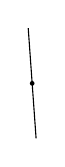
\begin{tikzpicture}\draw (0,-.7)--(-.1,.7);\fill (-.05,0) circle (.03);\end{tikzpicture}}
\diagram{\begin{tikzcd}[ampersand replacement=\&,column sep=small,row sep=large]
\widehat{\mathscr O}_x\otimes_{\mathscr O_x}({\unsure{m|\mathfrak m}}^n/m^{{\unsure{n+1|n}}})_{{\unsure{v|\nu}}}\arrow[r]\&\widehat{\mathscr O}_x\otimes L_{{\unsure{n+1|u n}}}\arrow[r,dash]\&\widehat{\underline{\mathscr O}}_x\otimes L_n\\
\&\widehat{\mathscr O}_{\deleted{{\unsure{x}}}}/m^{n+1}\arrow[u,"*\quad *"]\arrow[r]\&\widehat{\mathscr O}_{\deleted{x}}/m^n\arrow[u,"*"]\\
\&*\&*
\end{tikzcd}}
\diagram{\begin{tikzcd}[ampersand replacement=\&,row sep=small]
k[[s,t]]\&\\
k[s,t]\arrow[u]\arrow[r]\&k[s,t]_{(s)}\\
m\&
\end{tikzcd}}
\[\deleted{{\unsure{K|t}}}\qquad\begin{array}{ccc}x_0&x_0&x_0\\x_1&x_1&\deleted{{\unsure{x_1|x}}}\\x_{{\unsure{1|2}}}&x_{{\unsure{1|2}}}&x_1\\&x&x_2\end{array}\]
\margin{$\prod\widehat{\underline{\mathscr O}}_x$}
% margin note written sideways
\margin{$(\widehat{\underline{\mathscr O}}_x^{\deleted{*}}\otimes_{\mathscr O_x}K)^*$}
% margin note written sideways
\diagram{\begin{tikzcd}[ampersand replacement=\&,row sep=large]
k[s]\\
\begin{array}{c}x_0\\x_2\end{array}\arrow[u]
\end{tikzcd}}
\[\widehat{\mathscr O}_{{\unsure{x|2}}}\deleted{{\unsure{\otimes_{\mathscr O_x}}}}{\unsure{\varpi|\pi|\mathfrak p}}\mathscr O_v/\varpi\mathscr O_v-\widehat{\mathscr O}_x\otimes_{\mathscr O_v}\varpi\mathscr O_v/\varpi^{{\unsure{2}}}\mathscr O_v-\widehat{\mathscr O}_x\otimes_{\mathscr O_v}L\]
\diagram{\begin{tikzcd}[ampersand replacement=\&,row sep=small]
{\unsure{\mathscr A|\mathcal A}}_{i_0--i_{p-1}}\arrow[d]\&\\
\mathscr A_{i_0---i_p}.\&\mathscr A_{i_p}\arrow[l]
\end{tikzcd}}
\[\widehat{\mathscr O}_{{\unsure{u|x}}}\longrightarrow\widehat{\mathscr O}_x\ S^{-1}\]
\[\varpi\qquad\varpi^2\]
\figure{\begin{tikzpicture}\draw[thick] (0,0) ellipse (.45,.35);\draw(-.1,-.34)..controls(.1,0)and(0,.2)..(-.1,.34);\draw(-.6,.2)..controls(-.3,0)and(.3,-.2)..(.43,-.05);\end{tikzpicture}}
\[k[[t]][\deleted{{\unsure{s}}}s]/(s^{{\unsure{n}}}\]
\margin{$k[[s,t]]$}
% margin note written sideways
\[\mathscr A_{[p_0,--p_n]}\otimes_A A_{p_{n+1}},{\unsure{p_{n-1}|p_{n+1}}},A_{p_n}\]
\margin{-- {\unsure{localiser}} en les {\unsure{polynômes}} en $s,t$ qui {\unsure{ne sont pas}} {\unsure{multiples}} de $s$}
\[a_0(t)+a_1(t)s{\unsure{\sim|\cdots}}+a_{n-1}(t)s^{n-1}\]
\[a_0(t)[1+a_0(t)^{-1}a_1(t)s\sim\]
\[A_{[p_0]}\widehat\otimes_A\underline{A_{[p_1]}}\]
\[\widehat{\mathscr O}_x\otimes K\]
\diagram{\begin{tikzcd}[ampersand replacement=\&,row sep=large]
\deleted{a_0}\quad k((t))[s]/(s^n)\\
k[[s,t]]\arrow[u]
\end{tikzcd}}
\[\mathscr A_{\ell_0,\ell_1,\ldots,\ell_p}\qquad\mathscr A_{\ell_{p+1}}\qquad\mathscr A_{{\unsure{\ell|2}}}\]
\figure{\begin{tikzpicture}\draw (0,1.2)..controls(.8,.4)and(1,-.2)..(1.15,-1);\draw(.65,-.35)..controls(1,-.1)and(1.3,-.05)..(1.4,-.12);\node at (1.15,-1.25) {$s=0$};\end{tikzpicture}}
\[\underline{\underline{a_0(t)}}+\underline{\underline{a_1(t)}}s\sim+\underline{\underline{a_{n-1}(t)}}s^{n-1}\]
\[\mathscr A_1\qquad\mathscr A_{[{\unsure{X|x}}]}^{\otimes}\]
\[\mathscr O_x\quad\mathscr A_0\quad\otimes.\]
\[\varprojlim\widehat A\otimes_A A/{\unsure{\mathfrak m_i|\mathfrak n_i|\pi_i}}\]
\[\varprojlim A\]
\[\begin{aligned}k((t))[[s]]\\k[[t]][[s]]\\k((t))/k[[t]]\qquad[[s]]\end{aligned}\]
